\chapter{Kinematics}

Kinematics is the study of motion without concerning its cause. It allows
us to calculate and find out the evolution of a body. Everything in our world undergoes
motion, one way or the other. To begin our study of motion, let us first
concern ourselves with some definitions.

\section{Reference Frame and Point Particle}

Motion of any object is considered to relative to an observer. The observer defines
a particular co-ordinate system called the reference frame

\begin{figure}[ht]
        \centering
        \incfig{3daxes}    
    \caption{A Reference Frame}\label{fig: 3daxes}
\end{figure}

We use a reference frame according to our convenience. In general, we use the 3-dimensional cartesian system like the one
in \cref{fig: 3daxes}.

\index{Reference Frame}

\begin{definition}
    [Reference Frame]
    A reference frame is a co-ordinate frame relative to which motion of a particle is considered.
\end{definition}

We shall, until we encounter rigid body systems consider the motion of a point particle. 
Well, why? It is done so to simplify the calculation of our system. The motion of a (rigid)body is discussed later.

\index{Particle}
\begin{definition}
    [Point Particle]
    A particle whose size is negligible in the study of its motion is called a point particle.
\end{definition}

To discuss the motion, state of our body, it is also necessary to setup some time co-ordinate.
It is the reading of the clock in the observer's frame. In general, we setup our clocks
at \(0\) at the start of an event.

\section{Position Vector and Displacement}

\subsection{Position Vector}
\index{Position Vector}

\marginnote{One thing of importance is that a position vector of a particle is a function
of time. We generally denote this as \(r(t)\) to show that is a function.}

We define the position of a particle relative to a reference frame using a \emph{position 
vector}. One end of the position vector is the origin of our reference frame. The other is 
the particle itself. Consider \cref{fig: position}, the 
vector \(\vec{r}\) from \(O\) to \(A\). It describes the position of \(A\) relative to the
co-ordinate frame. Let \(A = (x,y,z)\). Then we denoted \(\vec{r}\) as \(\vec{r}(x,y,z)\).

The position to any point is written as, \[
    \vec{r} = (x,y,z) = x\unitv{i} + y\unitv{j} + z\unitv{k}
\]

\begin{figure}
    [H]
    \centering
    \scalebox{0.8}{\incfig{position}}
    \caption{A position vector, \(\mathbf{r}\).}
    \label{fig: position}
\end{figure}

\subsection{Displacement}
\index{Displacement}

\marginnote{Note that the position vector is not a \emph{true} vector. It is tied to particular
    reference frame.}

Consider the movement of a particle from \(A = (x_1,y_1,z_1)\) to \(B = (x_2,y_2,z_2)\). 
The \emph{displacement} is the change in the position vector,
and defines a true vector \(\vec{s} = (x_2-x_1,y_2-y_1,z_2-z_1)\).
\(\vec{s}\) is called the displacement vector. 
Note that it contains no information about the
individual positions, but only about the relative position of each. Thus, our choice
of reference frame, and thus position vector does not matter when we're concerned with displacement. 
In \cref{fig: displacement}, the vector
\(\vec{S}_{AB}\) defines a displacement from \(A\) to \(B\).

\begin{figure}
    [H]
    \centering
    \scalebox{1}{\incfig{displacement}}
    \caption{Displacement from \(A\) to \(B\)}
    \label{fig: displacement}
\end{figure}

The difference between displacement and distance is that of the path they describe. The distance covered is the length
of the actual path, while the magnitude of the displacement is simply the length of the vector between the final and initial positions.

\begin{marginfigure}
    \centering
    \scalebox{2.4}{\incfig{distance}}
    \caption{Distance}
\end{marginfigure}

\begin{algorithm}
    Consider the case of displacement and distance of a particle in circular motion with radius \(r\) Let it move from \(A\) to \(B\), inscribing
    an angle \(\theta\) (in radians) Then, we have,\\
    ~\\
    Distance between \(A\), \(B\) = \(r\theta\)\\
    Displacement between \(A\), \(B\) = \(2r\sin\left(\dfrac{\theta}{2}\right)\)
\end{algorithm}

\begin{figure}
    [H]
    \centering
    \incfig{distdisp}
    \caption{Displacement in a circle}
\end{figure}

\section{Speed and Velocity}

\index{Speed}

We are already familiar with the notion of speed. In elementary terms, speed is \({distance}/{time}\).
Speed itself is an elementary concept. It tells us nothing about the direction of the object whose speed we are
talking into consideration. Thus, it is a \emph{scalar} quantity.

\parbreak
\marginnote{The symbol \(\equiv\) stands for `defined as'.}

\index{Velocity}

The Velocity of a particle, contrastingly, contains information about both the speed and direction of the
object in consideration. It is a vector. Similar to position, it is also generally a function of time \(v(t)\), though it
may also be dependent on the position \(v(x)\).

\begin{definition}
    [Velocity]
    \label{def: velocity}
    Velocity is defined as,
    \begin{equation}
        \vec{v} \equiv \ndiv{\vec{r}}    
    \end{equation}
\end{definition}

One thing of note is that velocity can also be expressed as the derivative of 
displacement, which is just \(\vec{r} - \vec{r}_0\). Since the latter 
term is constant, we simply get that \(\ndiv{\vec{s}} = \ndiv{\vec{r}}\).

From this definition, we may gather that,

\[\int_{r_0}^{r} \dd{\vec{r}} = \int_{0}^{t} \vv \dd{t}\]

Or, 
\begin{equation}
    \vec{r} = \vec{r}_0 + \int_{0}^{t} \vv \dd{t}
\end{equation}

Sometimes, we do not need to compute the derivative of the position vector, and simply need an average
estimate, or in the case of uniformly accelerated motion, it is not required that we computer derivatives.
In such a case we use the concept of \textbf{average velocity}, \[
    \bavg{\vec{v}}_{12} = \frac{\increment\vec{s}}{t_2 - t_1}  
\]

\marginnote{The dot over \(r\) in \(\dot{\vec{r}}\) tells us that \(r\) has been differentiated
with respect to time.}

\begin{algorithm}
    Let us consider the cases of average velocity,
    \begin{casework}
        \ii When there are \(n\) equal time intervals with velocity \(\vec{v}_1, \vec{v}_2, \ldots, \vec{v}_n\).
        Then, \[
            \bavg{\vec{v}} = \frac{\vec{v}_1 + \vec{v}_2 + \dots + \vec{v}_n}{n} 
        \]
        \ii When there are \(n\) equal intervals of distance/displacement with velocity \(\vec{v}_1, \vec{v}_2, \ldots, \vec{v}_n\).
        Then, \[
            \bavg{\vec{v}} = \frac{n}{\frac{1}{\vec{v}_1} + \frac{1}{\vec{v}_2} + \dots + \frac{1}{\vec{v}_n}} 
        \]
    \end{casework}
\end{algorithm}


In general velocity is also referred to as `instantaneous velocity'. This is done to remind of the difference
with average velocity. We will not refer to it that way since by velocity we shall always mean \(\vec{v}\) as defined in
\cref{def: velocity}. The same goes for speed. Notably, speed is not defined as \(\ndiv{d}\) where \(d\) is the distance.

While the average speed is very well that, speed is actually the magnitude of the velocity of that point. 
Consider the distance between \(a\) and \(b\) as 
\(a \to b\). The path between them approaches a straight line. Thus, the distance and displacement become the same
in the limiting case. Therefore, the \emph{magnitude} of velocity is the speed at that instant.

Therefore, 

\[\text{speed} = \abs{\dv{\vec{r}}{t}}\]




\begin{algorithm}
    Let us consider some techniques for solving equations of velocity. Consider the case when velocity and time are given
    and we have to figure out displacement or when displacement and and velocity are given, but time is not. 
    \begin{enumerate}
        \ii \(v = c\) : This is a trivial case. Just use equations of uniformly accelerated motion.
        \ii \(v = f(x)\) : \(\displaystyle \dv{x}{t} = f(x)\). Then, \(\dfrac{\dd{x}}{f(x)} = \dd{t}\).
        Now, we simply have, \[
            \int^{x_2}_{x_1} \frac{\dd{x}}{f(x)} = \int^{t_2}_{t_1} \dd{t}
        \] to get \(x_1\) and \(x_2\) or \(t_1\) and \(t_2\). We may also set our co-ordinates such that \(x_2 = x\), \(x_1 = 0\) and \(t_2 = t\), \(t_1 = 0\).
        \ii \(v = f(t)\) : This is also easy, just, \(\displaystyle f(x) = \dv{x}{t}\), then,
        \[
            \int^{t_2}_{t_1} f(t) \dd{t} = \int^{x_2}_{x_1} \dd{x}
        \] We simply get \(x_1\) and \(x_2\) or \(t_1\) and \(t_2\) by solving the integral.
    \end{enumerate}
\end{algorithm}

\section{Acceleration}

If a body does not move with uniform velocity, it accelerates. Acceleration is also a vector and
is the rate of change of velocity.

\index{Acceleration}

\begin{definition}
    [Acceleration]
    \label{def: acceleration}
    Acceleration is defined as,
    \begin{equation}
        \vec{a} \equiv \ndiv{\vec{v}} = \nddiv{\vec{r}}    
    \end{equation}
\end{definition}

Much like the velocity definition, we have,

\begin{equation}
    \vv = \vv_0 + \int_0^t \vec{a} \dd{t}
\end{equation}

There is also another way to represent acceleration, as, \[
    \vec{a} = \vec{v}\dv{\vec{v}}{x}
\]

Such a representation is particularly useful when the velocity of a particle 
is a function of its position. In such a case, derivating with time is quite a hassle.

\section{Uniformly Accelerated Motion}

When the acceleration of a particle, \(a\) is constant, it undergoes uniformly accelerated motion.
We use special cases of integrals of \(a\) and \(v\) with respect to time and position for deriving
the equations of importance.

\begin{theorem}
    For a particle with initial velocity \(u\) undergoing uniformly accelerated motion of acceleration \(a\),
    \begin{align}
        v &= u + at \\
        v^2 &= u^2 + 2as \\
        s &= ut + \frac{1}{2} at^2 \\
        s_{n} &= u + \frac{a}{2}(2n - 1)
    \end{align}
\end{theorem}

\para{The derivation of these is quite easy, integrate \(\int a \dd{x}\) for the first, 
\(\int a \dd{t}\) for the second (both with constant acceleration), substitute from the former into the latter for the third,
and finally for \(n^{th}\) second just do \(s_n - s_{n-1}\).} 

\para{Now, we will be looking at some fascinating questions that I have encountered.}

\begin{example}
    Consider a particle moving with acceleration \(\alpha\) initially. After some time, it starts
    to `de-accelerate' at \(\beta\) acceleration. After time \(t = T\), the particle comes to a stop.
    Find the displacement covered by particle in time \(T\).
\begin{soln}
        It might be tempting to start calculating after setting up time \(t = t_0\) when acceleration
        changed from \(\alpha\) to \(\beta\), i.e., the particle moves with acceleration \(\alpha\) till
        \(t = t_0\).\\
        However, let us try to do a cleaner solution. Consider the \(v-t\) graph of the particle,

        \begin{figure}
            [H]
            \centering
            \begin{tikzpicture}
                \begin{axis}[funcgraphbare, xmax=5.8, ymax=10, xlabel={$t$}, ylabel={$v$}]
                    \addplot[red,domain=0:3]{3*x} node[left,pos=1/2] {$\alpha$};
                    \addplot[blue,domain=3:4.8]{(-5)*x+24} node[right,pos=1/2] {$\beta$};
                    \draw [black,dashed] (axis cs:3,0)--(axis cs:3,9) node[left,pos=1/25] {$t_0$};
                    \draw [black] (axis cs:4.8,-1)--(axis cs:4.8,0.5) node[right,pos=1] {$T$};
                    \draw [black,dashed] (axis cs:0,9)--(axis cs:4.8,9) node[right,pos=1] {$v_{max}$};
                \end{axis}
            \end{tikzpicture}
        \end{figure}
        Note that \(\alpha(t_0) = \beta(T-t_0) = v_{max}\). Thus,
        \begin{align*}
            \alpha(t_0) &= \beta(T-t_0) \\
            \alpha(t_0) &= \beta(T) - \beta(t_0) \\
            \alpha(t_0) + \beta(t_0) &= \beta(T) \\
            t_0 &= \frac{\beta T}{\alpha + \beta} \\
            v_{max} &= \alpha t_0 \\
            v_{max} &= \frac{\alpha\beta T}{\alpha + \beta}
        \end{align*}
        Now, note that \(\dfrac{1}{2} \times v_{max} \times T\) is the area under the graph.
        \begin{moral}
            The area under the \(v-t\) is the total displacement.
        \end{moral}
        Thus, displacement, \(s = \dfrac{\alpha\beta T^2}{2(\alpha + \beta)}\).
\end{soln}
\end{example}

\begin{example}
    A car is at distance \(d\) from a boy. It starts accelerating at \(a\) \unit{\metre\per\second\squared}. What is the minimum velocity that the boy should
    have to catch up with the car.
    \begin{soln}
        Consider separation of boy and car, \(s_{c,b}\). Using the equations of motion, 
        we have \(s_{b} = vt\), \(s_{c} = \dfrac{1}{2}at^2\). Thus, 
        \begin{equation}
            \label{eq: vel}
            s_{c,b} = d + \frac{1}{2}at^2 - vt        
        \end{equation}
    
        The most important thing to note here is that, 
        \begin{moral}
            For two objects to meet, the solution for time must be real.
        \end{moral}
        Therefore, from the simple equation, \eqref{eq: vel}, we must have, for real solutions,
        \(b^2 - 4ac\) for the equation \(at^2 + bt + c\). Solving for this by substituting values from
        \eqref{eq: vel}, we have,
            \begin{equation}
                v \ge \sqrt{2ad}
            \end{equation}
    \end{soln}
\end{example}

\begin{remark}
    One thing of note is that the converse of above is true as well,
    \begin{moral}
        For two objects to \emph{not} meet, the solution of time must be imaginary or negative.    
    \end{moral}
\end{remark}

\para{One more key note to takeaway is that,}

\begin{moral}
    At instant of maximum separation, relative velocity of particles is \(0\).
\end{moral}

\begin{example}
    A body is dropped at \(t = 0\), after time \(t = t_0\), another body is thrown downwards with
    velocity \(u\) \unit{\meter\per\second}. Assuming first body reaches ground first, plot graph
    of separation.

    \begin{soln}
        At instant \(t_0\), displacement of first particle = \(\dfrac{1}{2}gt_{0}^2\). Note that here
        we set up co-ordinates such that positive \(y\) is downwards from point of drop. The displacement 
        of first body at \(t = t\) after \(t_0\) but before \framebox{reaching ground} is
        \begin{equation}
            s_1 = \frac{1}{2}gt_{0}^2 + \frac{1}{2}g(t-t_0)^2
        \end{equation}
        While for second body is,
        \begin{equation}
            s_2 = ut + \frac{1}{2}g(t-t_0)^2
        \end{equation}

        Thus, 
        \begin{equation}
            s_{1,2} = \frac{1}{2}g(t_0)^2 + t(gt_0 - u)
        \end{equation}

        Thus, before reaching ground, \(s-t\) graph is linear. However, after first body reaches ground,

        \begin{equation}
            s_{1,2} = ut + \frac{1}{2}g(t)^2
        \end{equation}
        which is a parabola. Thus, overall graph is,
        \begin{figure}[H]
            \centering
            \begin{tikzpicture}
                \begin{axis}[funcgraphbare, xlabel={$t$}, ylabel={$s$}]
                    \addplot[red, domain=0:2] {x+2};
                    \addplot[red,domain=2:3] {1.5*(-x^2)+5*x};
                \end{axis}
            \end{tikzpicture}
        \end{figure}
    \end{soln}
\end{example}

\begin{example}
    Find the total displacement if the \(v-t\) graph is as follows,
    \begin{figure}
        [H]
        \centering
        \begin{tikzpicture}
            \begin{scope}[xshift=10cm]
                % Axes
                \draw (0,0) node[below left] {$O$}
                    (0,0) -- (7,0) node[below] {$t$}
                    (0,-0.5) -- (0,3.5) node[left] {$v$};
                
                \draw (6.4,0) arc[start angle=0, end angle=180, radius=3.2];
            \end{scope}
        \end{tikzpicture}
    \end{figure}
    The idea behind this is simple, the graph here is \textbf{not} a semicircle. It is an
    ellipse, because of dimensional limitations! The equations of circle, \(v^2 + t^2 = r^2\)
    doesn't work because we cannot add two dimensionally different quantities.

    Therefore, the graph is an ellipse, and we conclude by computing the area of the ellipse. I haven't
    given the data, since I wanted to mention the idea.
\end{example}

\section{Motion in Polar Co-ordinates}

The polar co-ordinate axes are the two-dimesional subset of the 3-d cylindrical co-ordinates. 
Any point in polar co-ordinates is depicted by a system of two unit vectors, \(\unitv{r}\) and
\(\unitv{\theta}\). However, each of these are \framebox{dependent on the position of the particle} and
maybe written explicitly as \(\unitv{r}(\theta)\) and \(\unitv{\theta}(\theta)\).  

Here, \(\unitv{r}\) points in the direction of increasing radius(along the radial vector)
\(\unitv{\theta}\) points in the direction of increasing \(\theta\) (tangent to the radial vector).
These two unit vectors are \emph{orthogonal} at any point. 

\begin{figure}
    [H]
    \centering
    \incfig{polarunit}
    \caption{Unit vectors in polar co-ordinates}
    \label{fig: polarunit}
\end{figure}

\noindent In \cref{fig: polarunit} if \(\vec{r}\) makes
an angle \(\theta\) with the horizontal, then,

\begin{align}
    \label{eq: polardef}
    \unitv{r} &= \cos \theta \unitv{i} + \sin \theta \unitv{j}\\
    \unitv{\theta} &= -\sin \theta \unitv{i} + \cos \theta \unitv{j}
\end{align}

\section{Kinematics in Polar Co-ordinates}

Now let us formulate kinematics in polar co-ordinates. The position \(\vec{r}\) can be written as

\begin{equation}
    \vec{r} = r \unitv{r}
\end{equation}

\noindent Velocity follows normally, 
\begin{equation}
    \vec{v} = \ndiv{\vec{r}} = \ndiv{r} \unitv{r} + r\dv{\unitv{r}}{t} 
\end{equation}
or does it? What even is \(\displaystyle\dv{\unitv{r}}{t}\) ? Well the answer lies in 
the time-derivative of the unit vectors. Using the definitions in \eqref{eq: polardef}, we get,

\begin{align}
    \dv{\unitv{r}}{t} &= \ndiv{\theta} \unitv{\theta}\\
    \dv{\unitv{\theta}}{t} &= -\ndiv{\theta} \unitv{r}
\end{align}

\noindent Using these results, we get that

\begin{empheq}[box=\widefbox]{align}    
    \vec{v} & = \ndiv{r} \unitv{r} + r\ndiv{\theta} \unitv{\theta}\\
    \label{polar: accel}
    \vec{a} & = (\nddiv{r} - r\ndiv{\theta}^2) \unitv{r} + (r\nddiv{\theta} + 2\ndiv{r}\ndiv{\theta}) \unitv{\theta}
\end{empheq}

\noindent The most interesting result are the various terms of acceleration in \eqref{polar: accel}. First let 
us consider the terms along \(\unitv{r}\). \(\nddiv{r}\) is the \emph{radial} acceleration. It is
the change is radial speed. The second term \(-r\ndiv{\theta}^2\) is the \emph{centripetal} acceleration.
It arises from a change in tangential velocity.

Now let us consider the terms along \(\unitv{\theta}\). The \(r\nddiv{\theta}\) term is the tangential
acceleration resulting from change in tangential speed. The other term \(2\ndiv{r}\ndiv{\theta}\) is the
\emph{coriolis} acceleration. I shall discuss it when discussing rotating frames.

\section{Free Fall}

When an object is dropped downwards freely, it undergoes \emph{free fall}. We ignore
air resistance, until we're told not to and in general also talk about cases of the
object being thrown instead of dropped. An object dropped from any height undergoes
accelerations \(\vec{a}\) where \(\norm{\vec{a}} = g\). The direction and sign of acceleration
is entirely dependent on us.

In general, it is a good idea to setup our axes such that the direction above ground is positive
and towards the ground is negative. The acceleration during free fall is always towards
the ground. Therefore, for these cases \(\vec{a} = -g \unitv{j}\). 

Some important points of note are that ``\(g\)'' does not become positive or negative or whatever,
this is a common misconception. Instead, we just decide where exactly the positive direction is
and setup \(g\) according to that.
\parbreak
When a ball is thrown with some velocity \(u\) say in the positive directions
(change it into \(-u\) if in the negative direction), then we have,

\begin{algorithm}
    The following are special cases of equations of motion.
    \begin{enumerate}
        \ii \(v = u - gt\)
        \ii \(v^2 = u^2 -2gh\)
        \ii \(h = ut - \dfrac{1}{2}gt^2\)
    \end{enumerate} 
\end{algorithm}

The case when a ball is thrown upwards is exactly symmetrical to this one, but there
the ball goes up, reachs \(v = 0\) and then goes down. Also note that all of these equations are vector
equations.

\begin{example}
    Two balls are thrown in intervals of \(2\) seconds with velocity \(u\) each. Find the
    time when they collide.

    \begin{soln}
        Note that when they collide, their displacement from ground must be the same! Setting 
        the origin at ground, and direction of away from ground as positive, we have,
        
        For the first ball, \(h_{1} = ut - \dfrac{1}{2}gt^2\). Since the second ball
        is thrown \(2\) seconds later, \(h_{2} = u(t-2) - \dfrac{1}{2}g(t-2)^2\). Now, we just have
        \(h_{1} = h_{2}\) and the calculation is trivial.
    \end{soln}
\end{example}

The thing to note in this example is that you do not need to setup two cases, one in which
\(g\) is negative and one in which \(g\) is positive since it is in the direction of velocity. 
Just note that these equations are vectorial and we are done.

Some quick formulas to remember because they help a lot,

\begin{algorithm}
    For an object dropped from height \(h\),
    \begin{enumerate}
        \ii Time to reach ground, \(t = \sqrt{\dfrac{2h}{g}}\).
        \ii Velocity when it reaches ground \(v = \sqrt{2gh}\).
    \end{enumerate}
\end{algorithm}

Deriving them is easy, and they can be generalised as when it travels height \(h\) between
the point of drop to anywhere, instead of ground. Clearly, both still follow there.

Also, always remember,

\begin{moral}
    When an object is thrown/dropped from another object traveling with some velocity and
    acceleration, it inherits its velocity but not its acceleration.
\end{moral}

\section{Graphs in Motion}

In the graphs we are going to discuss, acceleration will either be \(0\) or constant.
These graphs help to quickly solve problems, especially related to total distance and 
displacement. 

Let us consider the direction away from origin positive, and towards origin negative.
Then, consider constant acceleration, \(a = c\). We have the following displacement time
graphs,

\begin{figure}[H]
    \centering
    \begin{subfigure}{0.5\textwidth}
        \centering
        \begin{tikzpicture}
            \begin{axis}
            [funcgraphbare, xlabel=$t$, ylabel=$s$]
            \addplot[red, domain=0:16]{x^2};
            \end{axis}
        \end{tikzpicture}
        \caption{For \(c > 0\). }
    \end{subfigure}%
    \begin{subfigure}{0.5\textwidth}
        \centering
        \begin{tikzpicture}
            \begin{axis}
            [funcgraphbare, xlabel=$t$, ylabel=$s$]
            \addplot[red, domain=0:16]{-x^2 + 256};
            \end{axis}
        \end{tikzpicture}
        \caption{For \(c < 0\)}
    \end{subfigure}%
\end{figure}

\section{Relative Motion}

There is a very neat technique to solve questions of kinematics, it is to switch our 
reference frames. Let the base reference frame be that of earth, then,

\begin{figure}
    [H]
    \centering
    \incfig{reference}
\end{figure}

If \(\vec{r}_1\) evolves with time, \(r_1(t)\). And so does \(r_2(t)\). Then,

\begin{align*}
    \vec{r}_1 &= \vec{r}_{1,2} + \vec{r}_2 \\
    \ndiv{\vec{r}}_1 &= \ndiv{\vec{r}}_{1,2} + \ndiv{\vec{r}}_2 \\
    \vec{v}_1 &= \vec{v}_{1,2} + \vec{v}_{2}\\
    \vec{v}_{1,2} &= \vec{v}_1 - \vec{v}_{2}
\end{align*}

Obviously if the vectors face the same direction in the same plane, then, the components subtract. If they face
opposite direction, then the components add. 

\(\vec{v}_{1,2}\) is called the velocity of \(\mathit{1}\) w.r.t \(\mathit{2}\). When doing
problems, try to setup a reference frame such that velocity of any single object vanishes.
This allows for a very neat simplification of problems. 

\section{Motion in higher dimensions}

We can mostly safely extend our results from one dimension to higher dimensions.
So for instances, velocity of a particle whose trajectory is defined as 
\(x\unitv{i} + y\unitv{j} + z\unitv{k}\) can simply be computed as,
\[v = \ndiv{x}\unitv{i} + \ndiv{y}\unitv{j} + \ndiv{z}\unitv{k}\] Such a thing
is not true for non-cartesian co-ordinates, as we say in the case of polar forms.
Due to the orthogonality of the cartesian unit vectors, and using dot products
we simply have, 
\[v_x = \ndiv{x}, v_y = \ndiv{y}, v_z = \ndiv{z}\]

And the same is true for all other vectors. This gives us the power to
resolve our vector components into components alongside unit vectors
and consider independent one dimensional motion for each of them.

\section{Projectile Motion}

Projectile motion is one of the most important motion to consider in 
2 dimensions. It is the motion of a projected body. Generally, we
only care about the motion of a body projected from ground under the influence
of gravity. 

Let a body be projected at an angle \(\theta\) from the ground at velocity \(\vec{v}\)
along \(\theta\). Then, by resolving \(\vv\) into \(v_x \unitv{i} + v_y\unitv{j}\),
we have, 
\begin{align*}
    x &= v_xt \unitv{i} \\
    y &= v_yt - \frac{1}{2}gt^2 \unitv{j}
\end{align*}

Doing some manipulations, we may note that \(v_x = v\sin(\theta)\), \(v_y = v\cos(\theta)\).
Also, substituting \(t = x/v\sin(\theta)\), we have,
\begin{equation}
    \boxed{y = x\tan(\theta) - \frac{gx^2}{2v^2\cos^2(\theta)}}
\end{equation}

The path of the projectile is parabolic as shown in \cref{fig: projectile}.

\begin{figure}[H]
    \centering
    \incfig{projectile}
    \caption{Trajectory of a projectile}
    \label{fig: projectile}
\end{figure}

Here, \(H\) is the maximum height of the particle. Clearly,
when the projectile is at \(H\), \(v_y = 0\). We have, 
\(v_y^2 = 2gH\),
\begin{equation}
    \boxed{H = \frac{u^2\sin^2(\theta)}{2g}}
\end{equation}

The time period of the projectile can be simply calculated as well,
since at the final time, \(T\), \(y = v_yt - 1/2gt^2 = 0\) and,

\begin{equation}
    \boxed{T = \frac{2v\sin(\theta)}{g}}
\end{equation}

\(R\) is the range the particle covers horizontally in time \(T\) and is
clearly,

\begin{equation}
    \boxed{R = \frac{v^2\sin(2\theta)}{g}}
\end{equation}

Note that if the particle is projected at \(\theta = \pi/4\), 
the range is maximum and is \(u^2/2g\). Otherwise,
for \(0 < \theta < \pi/2\), \(\sin(2\theta)\) attains the same 
value for two \(\theta_1, \theta_2\). These \(\theta_1\), \(\theta_2\) are complementary
by trigonometry.

More generally, if we consider the projectile to have an initial position of 
\(\qty(x_0, y_0)\), then, by substituting for time, we find that the 
vertex of the parabola is \(\qty(y_0 + \frac{u^2\sin^2\theta}{2g}, x_0 + \frac{u^2\sin2\theta}{g})\).

The range is a little more difficult to computer here, as the particle will transverse to 
the ground which is lower than \(y_0\). Freely setting up our co-ordinates 
as \(\qty(h, 0)\), we get by the equation of trajectory,

\[
    0 = h + R\tan(\theta) - \frac{gx^2}{2v^2\cos^2(\theta)}
\]

Derivating this with respect to theta to find the maxima, and then using the attained
value, we have, 

\begin{equation}
    R = \frac{u}{g}\sqrt{u^2 + 2gh}
\end{equation}

Some peculiar things about projectile motion is that, \begin{inparaenum}[a)]
    \ii it is reversible, and
    \ii the time to attain some vertical displacement can be found in terms of 
    the maximum height alone.
\end{inparaenum}

Consider the vertical position of the particle to be 
\(s\) at some time \(t\). Then, 
\[s = u_yt - \frac{1}{2}gt^2\] 
Also, note that if the maximum height is \(h\), 
\[u_y = \pm \sqrt{2gh}\]

Where the positive value is during the ascent and the negative is during the descent. Then,

\[s = \pm\sqrt{2gh}t - \frac{1}{2}gt^2\]

Solving for \(t\) gives us,
\[t = \pm \sqrt{\frac{2h}{g}} \pm \sqrt{\frac{2(h-s)}{g}}\]

If the initial velocity is positive and \(s > 0\), 

\begin{equation}
    t = \sqrt{\frac{2h}{g}} \pm \sqrt{\frac{2(h-s)}{g}}
\end{equation}
the two values correspond to the fact that the particle will have the same vertical
displacement at two instances of time.

If the initial velocity is positive but \(s < 0\), i.e the particle 
starts at some height but then transverses below it, 

\begin{equation}
    t = \sqrt{\frac{2h}{g}} + \sqrt{\frac{2(h-s)}{g}}
\end{equation}
is the only reasonable solution.

If the initial velocity is negative, then clearly the 
particle will attain a lower position. The maximum height in this 
case is simply the initial height of the particle.

\begin{equation}
    t = - \sqrt{\frac{2h}{g}} + \sqrt{\frac{2(h-s)}{g}}
\end{equation}

\section{Drag Forces}

In a more realistic scenario, a particle undergoing motion in any 
media experiences a \vocab{drag force}, anti-parallel to its velocity.
In particular,  

\begin{equation*}
    \vec{a} = -\alpha v \unitv{v} - \beta v^2 \unitv{v}
\end{equation*}

where the linear term arises from a property of the media, 
the viscosity(we will talk about it in the later sections.)

The quadratic term is a result of the collision of the particles with atoms 
and molecules during its motion. In general, 
the quadratic term dominates for higher velocities.

It is very difficult to analyse motion with drag, but we shall have a look at some particular 
cases of linear drag.

\marginref{\Cref{sec: newton's second law} \nameref{sec: newton's second law}}

\begin{example}
    Consider a projectile of mass \(m\) thrown upwards with initial velocity \(v_0\). It undergoes a linear drag 
    force, \(\Vec{F} =  -kv \unitv{v}\). Find the velocity of the particle as 
    a function of time. 

    \begin{soln}
        Using newton's second law, also by noting that 
        it also undergoes gravitation, \(\vec{a} = -g -kv/m \unitv{v}\).

        Now, we note that, 
        \begin{equation*}
            \dv{v}{t} = -g  - \frac{kv}{m}
        \end{equation*}

        \begin{align*}
            \frac{\dd{v}}{g + kv/m} &= - \dd{t} \\
            \int_{v_0}^{v_f} \frac{\dd{v}}{g + kv/m} &= \int_{0}^{t}\dd{t} \\
            \frac{m}{k} \eval{\log(g + kv/m)}_{v_0}^{v_f} &= t \\
        \end{align*}
        Which finally gives us,

        \begin{equation}
            v(t) = e^{-kt/m}v_0 + \frac{gm}{k}(e^{-kt/m} - 1)
        \end{equation}

    \end{soln}
\end{example}

The same idea can be extended to projectile --- \(2\)d motion 
by considering the components of the accelerations,

\[
    \vec{a} = -kv_x \unitv{i} - (g + kv_y) \unitv{j},
\]

and now considering the equations \(\dot{\vec{v}} = -kv_x\)
and the same for the \(y\) co-ordinate. 

Ulitmately, this leads to the equations,

\begin{align}
    v_x &= u_x e^{-kt} \\
    v_y &= \qty(u_y + \frac{g}{k})e^{-kt} - \frac{g}{k}
\end{align}

\section{Kinematics of a rigid body}

When we describe the motion of a point particle, we need \(3\) co-ordinates 
to do so in free space. For a system of \(n\) particles, we thus need
\(3n\) \emph{generalised co-ordinates}. This makes a description of motion
rather difficult.

However, when we concern ourselves with rigid bodies, the problem becomes
much easier. A rigid body is a system of particles such that they are 
always at a fixed distance apart from each other. For instance, 
the end points of a rod.

Rigid bodies, like everything in physics are a good approximation. 
The distances won't always be equal (for instance, at the time of collision).
But it is enough of an approximation that we'll let it go.

By Chasles' theorem, which we'll only state, we only \(6\) co-ordinates to 
describe a rigid body. Generally, we use \(3\) translational and \(3\) angular
ones.

Here, we're only going to look into the rotation of a rigid body.

Take an arbitrary point \(P\) on the body and set up cylindrical co-ordinates around it.
Which are polar co-ordinates with the \(z\) axis. We'll also set up an \(x-y\)
plane.
We note that the body rotates about \(P\) in such a frame.


In cylindrical coordinates, every point on the body can be ascribed a
coordinate \(\theta\), the angle between the projection of its position vector on the 
\(x-y\) plane. This is called the \vocab{azimuthal angle}.

The other two co-ordinates are \(r\), the distance of a particle from the 
\(z\) axis, and \(z\) the signed height of the body.

\begin{marginfigure}
    \centering
    \scalebox{0.4}{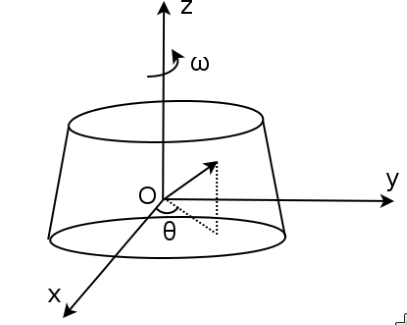
\includegraphics{../figures/rigidbody.png}}
    \caption{Rigid Body about \(P\)}
\end{marginfigure}

If a particle on a rigid body undergoes a change in its azimuth by \(\dd{\theta}\),
then because of the constraints of a rigid body, every particle 
undergoes a change of \(\dd{\theta}\). Thus, we define 
the angular speed of the rigid body, \(\omega\) to be \(\dv*{\theta}{t}\).

In the case of rigid body motion, we also define \(\vec{\omega}\), the \vocab{angular velocity}.
It has the magnitude \(\omega\) but points in the direction perpendicular 
to plane of rotation. We define the unique direction by the right hand grip rule. 
If you curl your fingers in the direction of rotation, then the direction 
in which your thumb points is the direction of \(\vec{\omega}\).

Consider a particle at a position \(\vec{r}\) from \(P\), and makes an angle
\(\phi\) with \(\vec{\omega}\). 

\begin{marginfigure}
    \scalebox{0.3}{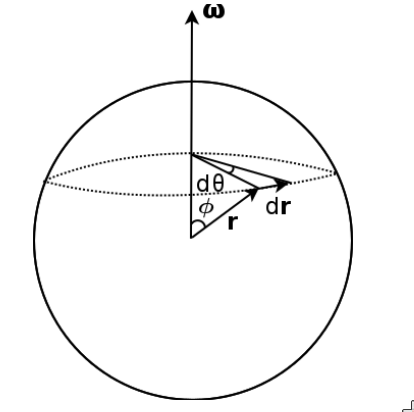
\includegraphics{../figures/rigidrotation.png}}
    \caption{\(\vec{\omega}\) and \(\dd{\vec{r}}\).}
\end{marginfigure}

Then, if it undergoes a change of \(\dd{\theta}\) azimuthally,
it moves through a circle of radius \(r\sin\phi\)
and transverses a distance \(\norm*{\dd{\vec{r}}} = r\sin\phi\dd{\theta} = r\sin\phi\,\omega\dd{t}\).

Thus, 

\[\dd{\vec{r}} = \vec{\omega} \cp \vec{r} \dd{t},\]

And, 

\begin{equation}
    \boxed{\dv{\vec{r}}{t} = \vv = \vec{\omega} \cp \vec{r}} 
\end{equation}

One thing we note across here is that if we take any another point on 
the rigid body, say \(Q\) which has a velocity \(\vv_Q\) in the frame of 
\(P\), then,

\[\vv_Q = \vec{\omega} \cp \vec{r}_{PQ}\]

In the frame of \(Q\), let us suppose that the body has an angular velocity, 
\(\vec{\omega}_1\). Then the velocity of \(P\) in the frame of \(Q\) must be 

\[\vv_P = \vec{\omega}_1 \cp \vec{r}_{QP} = -\vec{\omega}_1 \cp \vec{r}_{PQ}\]


Since \(\vv_P = -\vv_Q\) if \(Q\) is non-rotating,

\[\vec{\omega}_1 \cp \vec{r}_{PQ} = \vec{\omega} \cp \vec{r}_{PQ}\]

which gives us that \(\vec{\omega}_1 = \vec{\omega}\). This means that in any 
non-rotating frame with respect to \(P\), the angular velocity is the same.

\marginnote{\(\vec{\omega}\) is defined to be positive along the positive \(z\) axis.}

Basically, the angular velocity of a rigid body is intrinsic. It does not depend upon
the arbitrary point on the rigid body about which we establish our co-ordinates.

This is in contrast to something like the velocity which does depend on it. 

Generally, If the particle \(P\) has a velocity \(\vv_{ref}\) in the lab frame,
then the velocity of a point at a position \(\vec{r}\) from \(P\) in the lab 
frame is,

\begin{equation}
    \label{eq: velocity for rigid bodies}
    \vv = \vv_{ref} + \vec{\omega} \cp \vec{r}.
\end{equation}

\subsection{Instantaneous center of Rotation}

\Cref{eq: velocity for rigid bodies} can be seemingly simplified
by using a point known as the Instantaneous Center of Rotation, ICoR.

\begin{definition}
    The \vocab{Instantaneous Center of Rotation} is defined as the point that is fixed to the
    frame of the rigid body --- but not necessarily lying on the body --- that has
    zero velocity in the lab frame at that particular instant.
\end{definition}

The concept of being fixed to the ``frame'' of the body is a weird one. You may imagine 
it as something like a plane being attached to the body. This planes rotates with the body.
Now the ICoR is a point on the plane that has a \(0\) velocity in the lab frame. 

It does not, necessarily, lie on the body, but on the ``frame'' of the body, where it rotates just as the body does.
Of course, this talk to an attached plane is merely hypothetical. The ICoR lies 
on the extension of the body.

We may note that since the ICoR, which we shall denoted \(I\), has zero velocity in the lab frame, 
the velocity of any point \(P\) is simply,

\[\vv_P = \vec{\omega} \cp \vec{r}_{IP}\]

Thus the velocity at the point \(P\) is perpendicular to the line joining 
the ICoR and \(P\). 

For parallel velocities, thus, we may see that the ICoR lies on the line joining them.

\begin{marginfigure}
    \scalebox{2}{\incfig{icorpar}}
    \caption{ICoR for parallel velocities}
\end{marginfigure}

Here, 

\[v_A = \omega r_A, \, v_B = \omega r_B,\]

And, 
\[\frac{v_A}{r_A} = \frac{v_B}{r_A + d}\]

This allows us to greatly simplify and find for not only ICoR but the velocities 
from some type of argument to figure out the distances.

However, it is a bit more complicated for non-parallel velocities.

Consider \cref{fig: icornonpar}. The ICoR lies on the intersection point of the lines 
perpendicular to the velocity. Unfortunately, there is general way to calculate the 
ICoR and some geometric argument must be considered.

\begin{marginfigure}
    \scalebox{2}{\incfig{icornonpar}}
    \caption{ICoR for non-parallel velocities}
    \label{fig: icornonpar}
\end{marginfigure}

\subsection{Additive Property of Angular Velocities}

Angular velocities, much like velocities, are additive across
reference frames, i.e, for a rigid body \(B\), 

\begin{equation}
    \label{eq: angular velocities addition}
    \boxed{\vec{\omega}_{B1} = \vec{\omega}_{B2} + \vec{\omega}_{21}}
\end{equation}

Let us sketch out a proof of this. First, let us mention 
one extremely important equation that will be of much use, 

If a particle has velocities \(\vv_1\) and \(\vv_2\) in two
reference frames, the axes of frame \(2\) are rotating 
at \(\vec{\omega}_{21}\) with respect to the first frame
and \(\vec{r}_1\) is the position vector of the particle in the first
frame,

\begin{equation}
    \label{eq: rigidbody velocity accross rotating frames}
    \boxed{\vv_{1} = \vv_2 + \vec{\omega}_{21} \cp \vec{r}}
\end{equation}

While \cref{eq: rigidbody velocity accross rotating frames} bears 
a particular similarity to \cref{eq: velocity for rigid bodies}, they are 
very different.

\Cref{eq: rigidbody velocity accross rotating frames} tells us 
the velocity of a particle across two \textbf{rotating} frames,
while \cref{eq: velocity for rigid bodies} tells us the velocity 
of particle relative to the lab frame by using a reference point on the rigid body.

We won't prove this equation now but rather use it to prove \cref{eq: angular velocities addition}.

\begin{proof}
    Let \(R\) be the ICoR in the first reference frame.
    Then, for a rigid body \(B\) and the point on the body, \(P\),

    \[\vv_{P1} = \vec{\omega}_{B1} \cp \vec{r}_{RP}.\]

The velocity of \(P\) in frame \(2\) is, 

\[\vv_{P2} = \vv_{R2} + \vec{\omega}_{B2} \cp \vec{r}_{RP}.\]

Now, using \cref{eq: rigidbody velocity accross rotating frames} for \(\vv{R1}\), \(\vv{R2}\),

\[\vv_{R1} = \vv_{R2} + \vec{\omega}_{21} \cp \vec{r}_{R1},\]

where \(\vv_{R1} = 0\) because it is the ICoR. This gives us,

\[\vv_{P2} = \vec{\omega}_{B2} \cp \vec{r}_{RP} - \vec{\omega}_{21} \cp \vec{r}_{R1}\]

Finally, applying \cref{eq: rigidbody velocity accross rotating frames} for 
\(\vv_{P1}\) and \(\vv_{P2}\),

\[\vv_{P1} = \vv_{P2} + \vec{\omega}_{21} \cp \vec{r}_{P1},\]

And, 

\begin{align*}
    \vec{\omega}_{B1} \cp \vec{r}_{RP} &= \vec{\omega}_{B2} \cp \vec{r}_{RP} - \vec{\omega}_{21} \cp \vec{r}_{R1} + \vec{\omega}_{21} \cp \vec{r}_{P1} \\
    \vec{\omega}_{B1} \cp \vec{r}_{RP} &= \vec{\omega}_{B2} \cp \vec{r}_{RP} + \vec{\omega}_{21} \cp (\vec{r}_{R1} - \vec{r}_{P1}) \\
    \vec{\omega}_{B1} \cp \vec{r}_{RP} &= \vec{\omega}_{B2} \cp \vec{r}_{RP} + \vec{\omega}_{21} \cp \vec{r}_{RP}
\end{align*}

Since \(P\) was an arbitrary point, we can safely remove it, 

\begin{equation*}
    \vec{\omega}_{B1} = \vec{\omega}_{B2} + \vec{\omega}_{21}.
\end{equation*}

\end{proof}

\section{Angular Acceleration}

\begin{definition}
    The \vocab{angular acceleration} of a rigid body is the rate of 
    change of its angular velocity,
    \begin{equation}
        \vec{\alpha} = \ndiv{\vec{\omega}}
    \end{equation}
\end{definition}

Writing it more explicitly, 

\[\vec{\alpha} = \dv{\omega\unitv{\omega}}{t} = \ndiv{\omega}\unitv{\omega} + \omega\dv{\unitv{\omega}}{t}\]

For our purposes, we shall only consider \vocab{fixed axis rotation}. That is, rotation 
in which the direction of angular velocity does not change. 

Thus, 

\[\vec{\alpha} = \ndiv{\omega}\unitv{\omega} = \alpha\unitv{\omega}\]

The acceleration of an arbitrary point on the rigid body can be computed 
with respect to the lab frame with the help of another reference point on the 
body can be computed using \cref{eq: velocity for rigid bodies}.

\begin{equation*}
    \dv{\vv}{t} = \ndiv{\vv}_{ref} + \dv{\vec{\omega}}{t} \cp \vec{r} + \vec{\omega} \cp \dv{\vec{r}}{t} 
\end{equation*}

Here, \(\vec{r}\) is the position of the vector of the body relative to the reference point. 
Thus, it changes as \(\ndiv{\vec{r}} = \vv - \vv_{ref} = \vec{\omega} \cp \vec{r}\).

\begin{equation}
    \vec{a} = \vec{a}_{ref} + \vec{\alpha} \cp \vec{r} + \vec{\omega} \cp  (\vec{\omega} \cp \vec{r})
\end{equation}

This equation is general and valid for non-fixed axis rotation as well. 

For fixed axis rotation,

\begin{equation}
    \vec{a} = \vec{a}_{ref} + \alpha\unitv{\omega} \cp \vec{r} + \vec{\omega} \cp  (\vec{\omega} \cp \vec{r})
\end{equation}

If the rotation and translation of the body is strictly in a \(2\) dimensional plane,
the equation can be greatly simplified as \(\unitv{\omega} \cp \vec{r} = r\unitv{\theta}\)
(because \(\unitv{\theta}\) is along the direction of the cross product as \(\vec{r}\) and 
\(\vec{\omega}\) are perpendicular). 

\(\vec{\omega} \cp  (\vec{\omega} \cp \vec{r})\) can be simplified using the 
BAC-CAB rule, where, 

\begin{align*}
    \vec{\omega} \cp  (\vec{\omega} \cp \vec{r}) &= \vec{\omega}(\vec{\omega} \dtp \vec{r}) - \vec{r}(\vec{\omega} \dtp \vec{\omega}) \\
    \vec{\omega} \cp  (\vec{\omega} \cp \vec{r}) &= -\omega^2\vec{r} = -\omega^2r\unitv{r}
\end{align*}

Finally, we get, 

\begin{equation}
    \vec{a} - \vec{a}_{ref} = \alpha r \unitv{\theta} -\omega^2r\unitv{r}
\end{equation}

Just a point to remember is that we are taking \(\alpha\) as signed here, 
thus remember to use \(-\alpha\) if \(\alpha = -\alpha\unitv{\omega}\) in the equation.

